\documentclass[11pt]{article}

\usepackage[letterpaper,margin=0.75in]{geometry}
\usepackage{booktabs}
\usepackage{graphicx}
\usepackage{listings}

\setlength{\parindent}{1.4em}

\begin{document}

\lstset{
  language=Python,
  basicstyle=\small,          % print whole listing small
  keywordstyle=\bfseries,
  identifierstyle=,           % nothing happens
  commentstyle=,              % white comments
  stringstyle=\ttfamily,      % typewriter type for strings
  showstringspaces=false,     % no special string spaces
  numbers=left,
  numberstyle=\tiny,
  numbersep=5pt,
  frame=tb,
}

\title{Congestion Control: Part 2}

\author{Jonathan George}

\date{}

\maketitle

\section{Description}
This lab continues to explore the implementation of congestion control we implemented in the last lab. This lab mainly consists of experiments which show how TCP congestion control reacts to different circumstances.

\section{Basic Experiments}
This first section shows how TCP reacts to different flow amounts: 1,2, and 5. It uses a simple two node network. Each link has a bandwidth of 10 Mbps, propagation delay of 10 ms and 100 packet queue size. A 1 Mb file is transferred from n1 to n2. Three graphs are generated in each case: bps vs time, window size vs time, and queue size vs time. The queue size vs time graph also includes 'X' marks where packets are dropped due to queue overflow.

\subsection{One Flow}

Rate

\centerline{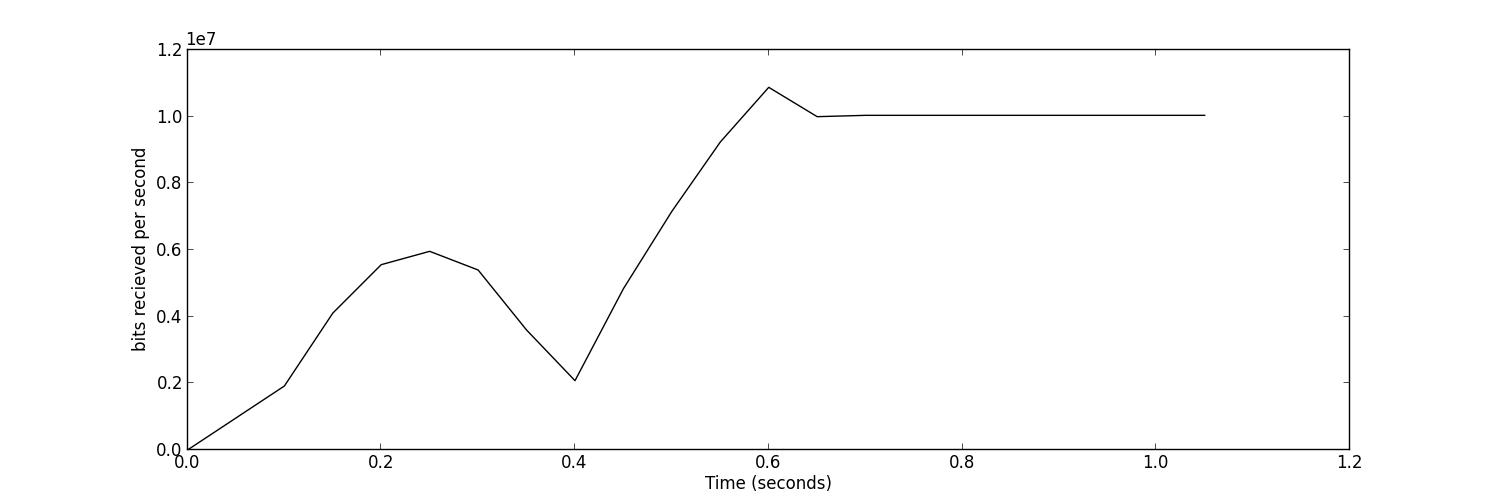
\includegraphics[width=22cm]{plot_rate_one.png}}

Window

\centerline{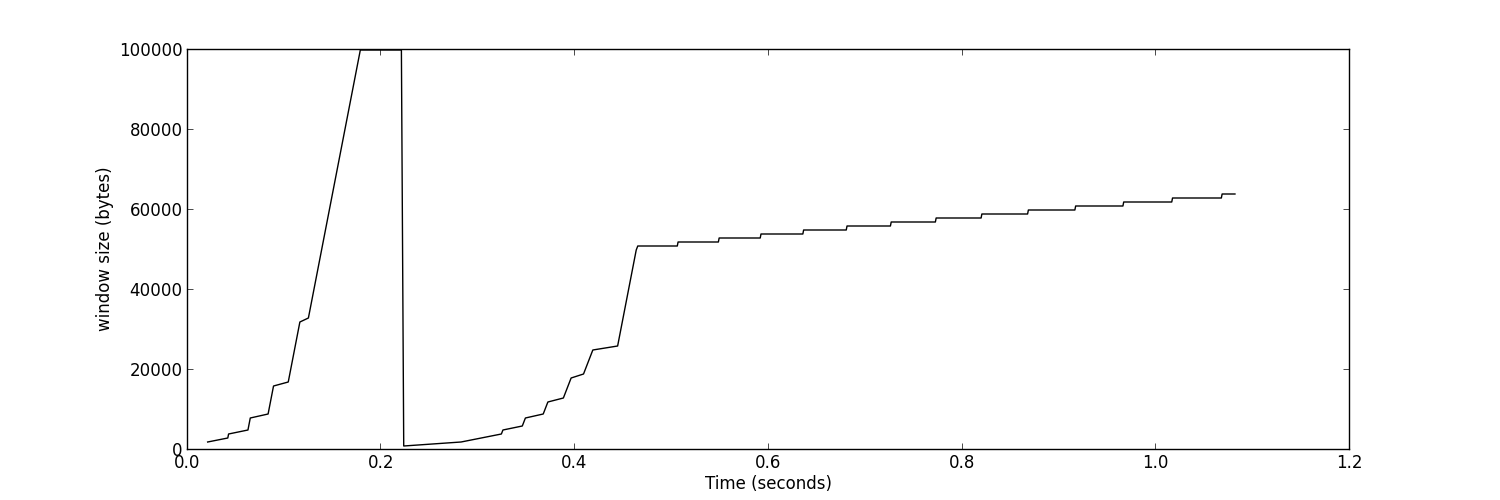
\includegraphics[width=22cm]{window_time_one.png}}

Queue

\centerline{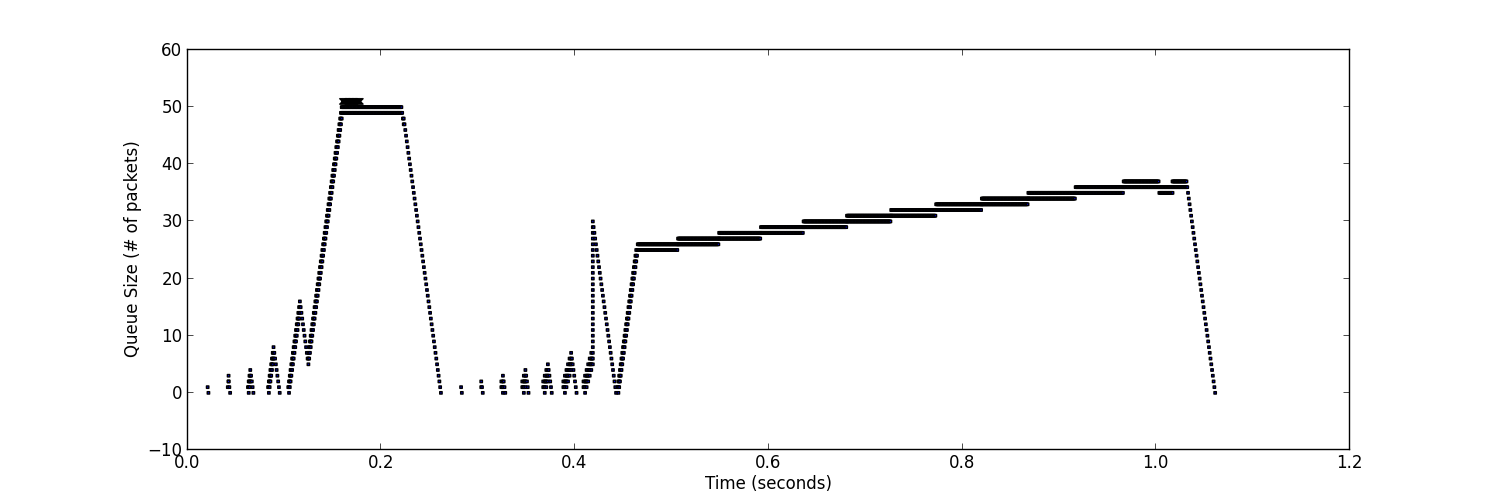
\includegraphics[width=22cm]{queue_time_one.png}}

As you can see from the three graphs above, the window size increased exponentially until reaching the queue filled up. It then experienced a loss event and restarted in slow start until it reached the threshold and then continued to increase slowly until the whole file was sent. It used most of the bandwidth towards the end.

\subsection{Two Flow}

In this section, the two flows were graphed together.

Rate

\centerline{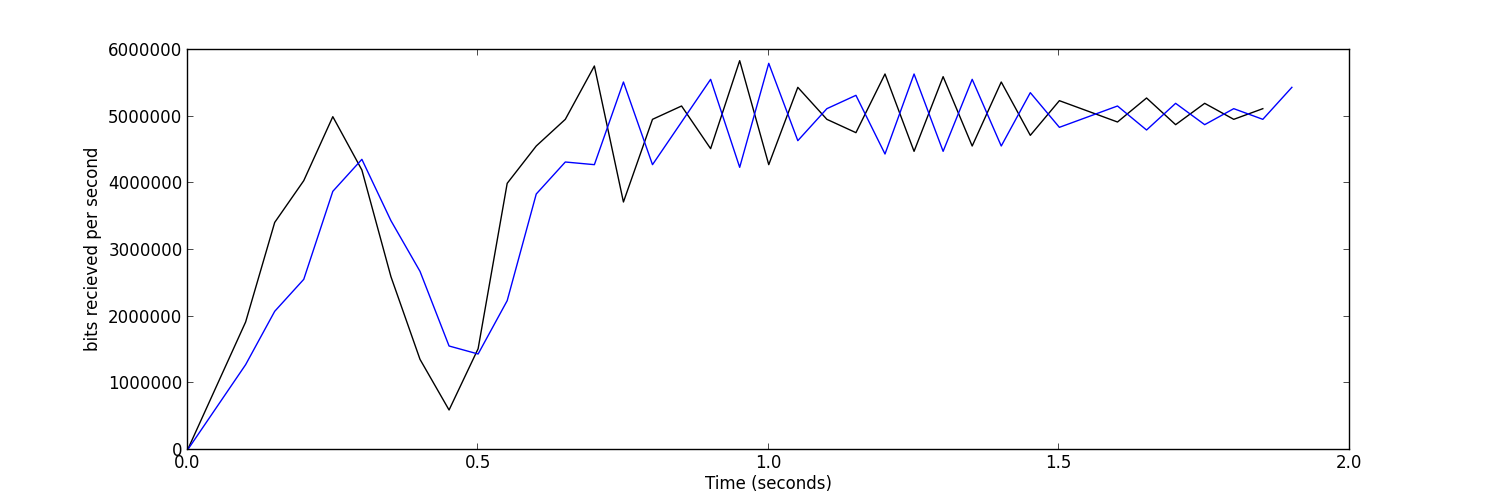
\includegraphics[width=22cm]{plot_rate_two.png}}

Window

\centerline{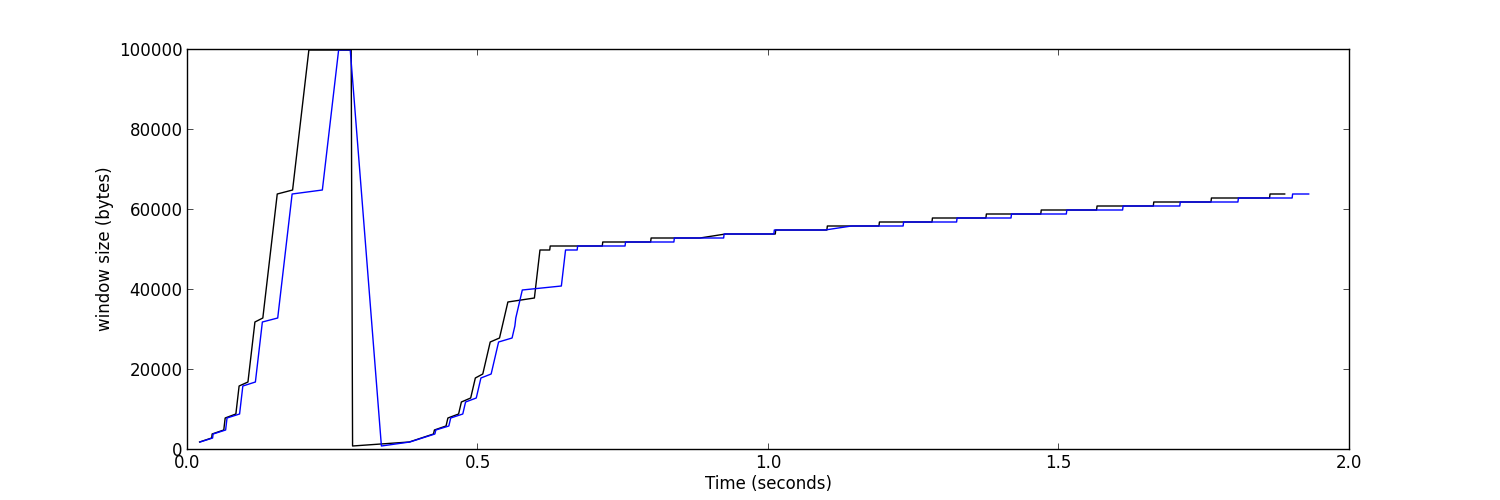
\includegraphics[width=22cm]{window_time_two.png}}

Queue

\centerline{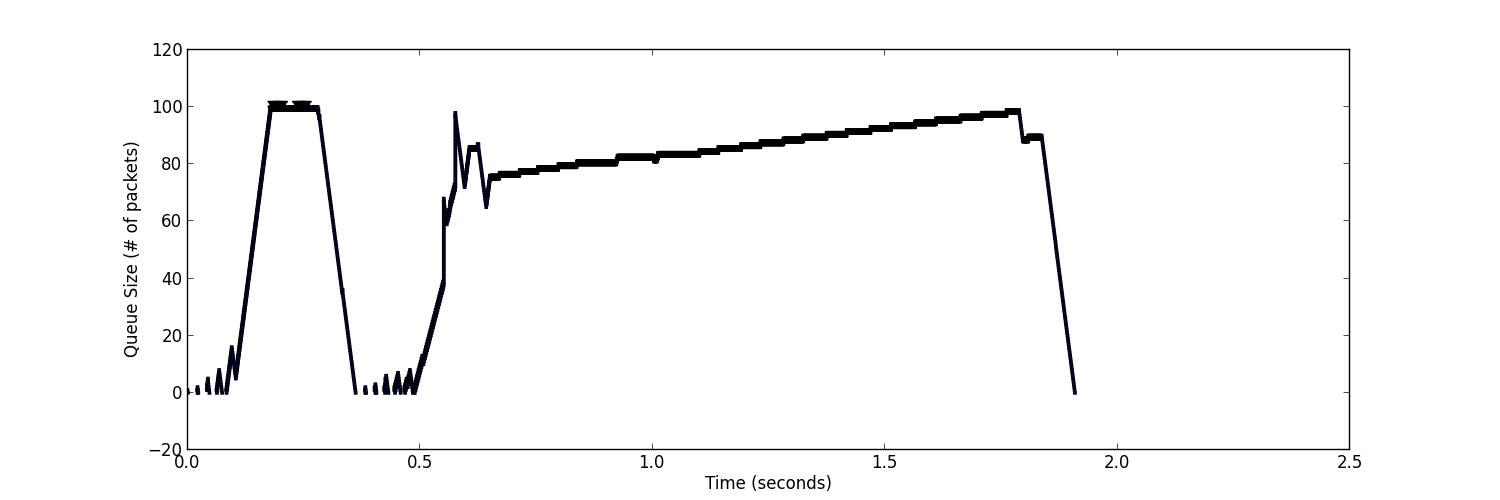
\includegraphics[width=22cm]{queue_time_two.png}}

As you can see in these graphs, the queue overflows pretty quickly and both flows have to back off. Over time they even out to both use about 50\% of the bandwidth.

\subsection{Five Flow}

In this experiment, we stagger the different flows in order to see how they will interact as one flow enters and another leaves.

Rate

\centerline{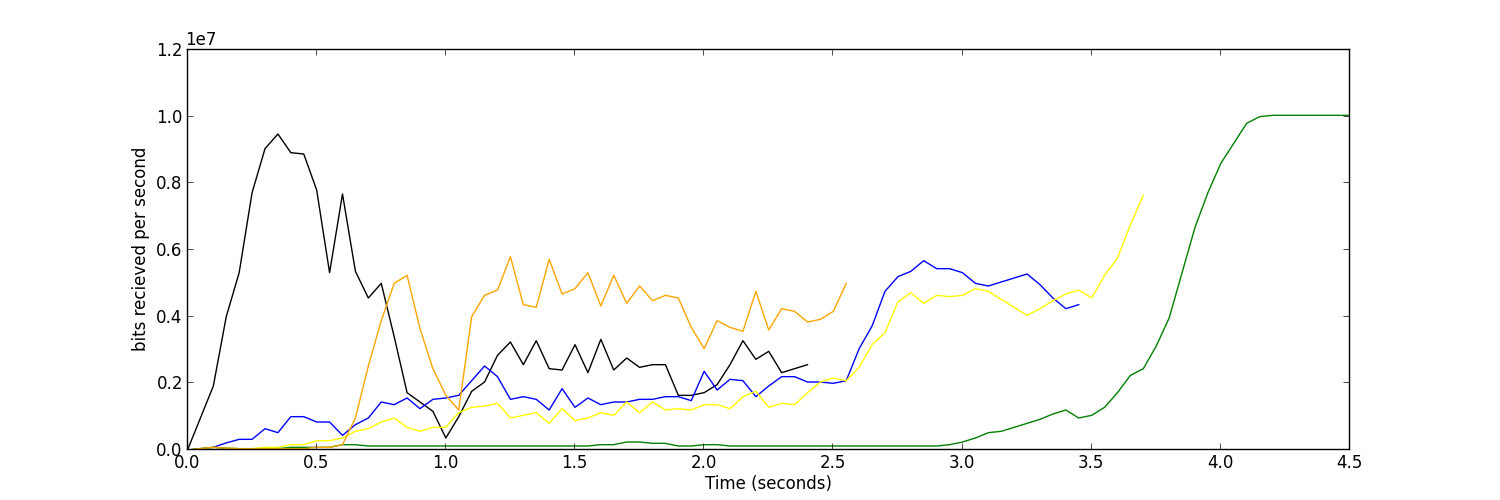
\includegraphics[width=22cm]{plot_rate_five.png}}

Window

\centerline{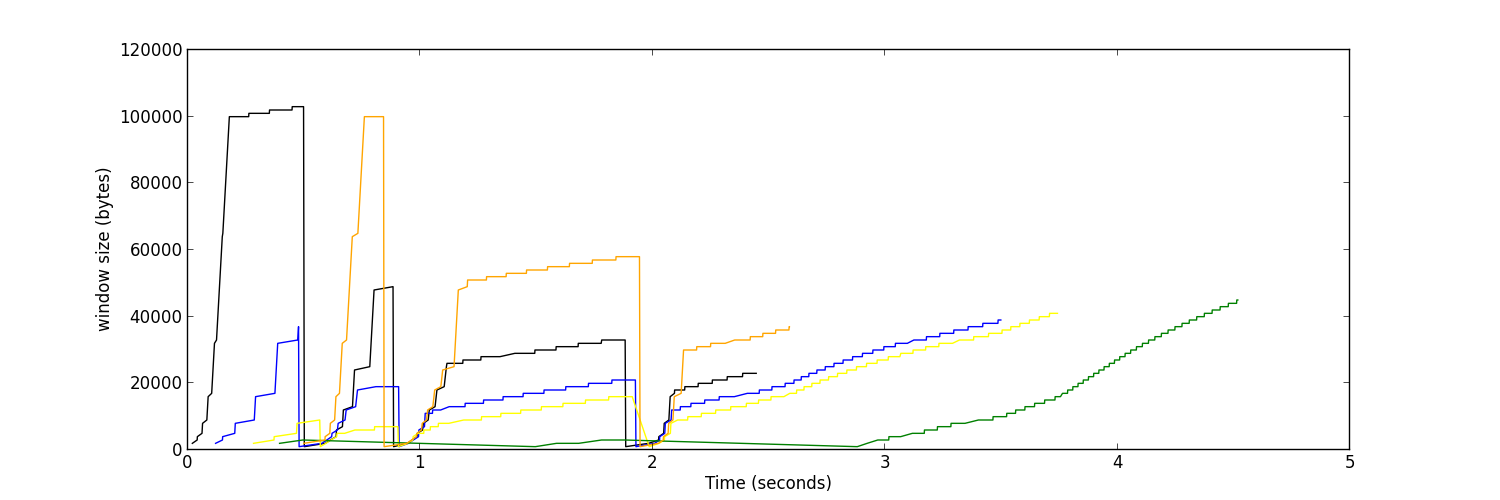
\includegraphics[width=22cm]{window_time_five.png}}

Queue

\centerline{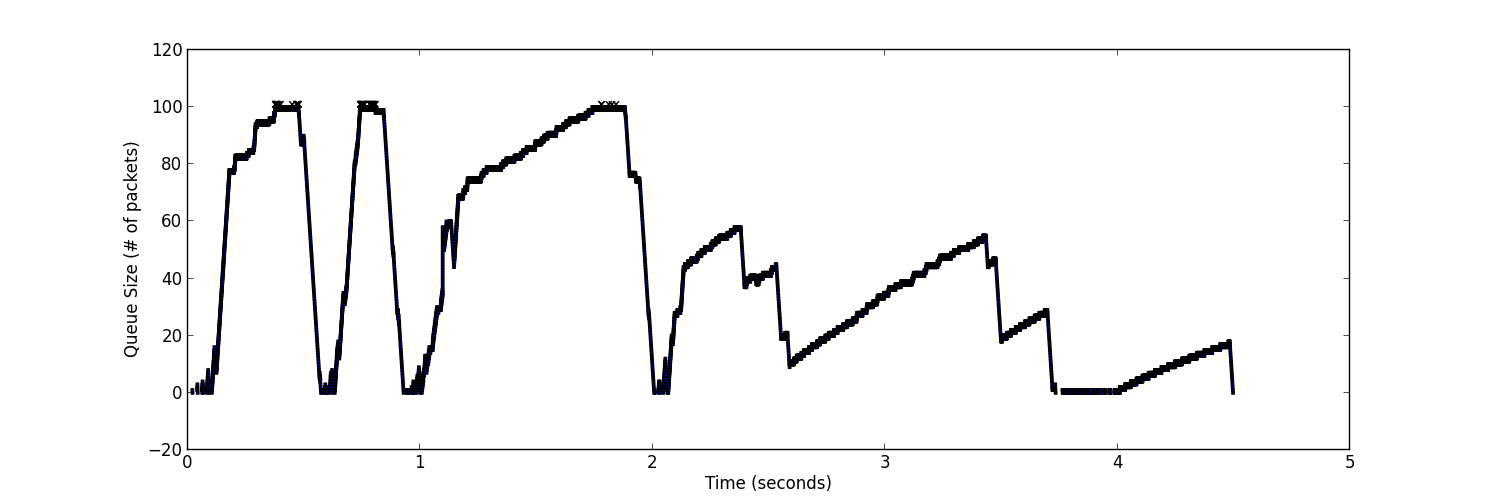
\includegraphics[width=22cm]{queue_time_five.png}}

As new flows start, they quickly grow larger than the other flows. However, once the queue overflows they drop down closer to the other flows. Over time, they find a good equilibrium. As a flow finishes, the other flows continue to grow and consume the bandwidth. This consumption of free bandwidth is pretty slow due to the additive increase of the window size. 

\section{Advanced Experiments}
In this section, we will examine different method of implementing fairness between flows.

\subsection{Additive Decrease}
This first section attempts to use additive decrease instead of multiplicative decrease to back off in the event of a loss.

Rate

\centerline{\includegraphics[width=22cm]{AIAD_rate_time.png}}

Window

\centerline{\includegraphics[width=22cm]{AIAD_window_time.png}}

Queue

\centerline{\includegraphics[width=22cm]{AIAD_queue_time.png}}

As can be seen the window size graph, additive decrease has a hard time finding a stable threshold level. This causes it to jump up and down quickly at first and eventually the threshold is sufficiently decreased that it calms down. This stabilizes eventually, but isn't as good as before.

\subsection{AIMD - 5/6th factor}
In this test, we changes the factor by which multiplicative decrease lowers the threshold by. Instead of setting the threshold to 1/2 of the window size, we set the threshold to 5/6th of the window size.

Rate

\centerline{\includegraphics[width=22cm]{AIMD_plot_rate.png}}

Window

\centerline{\includegraphics[width=22cm]{AIMD_window_time.png}}

Queue

\centerline{\includegraphics[width=22cm]{AIMD_queue_time.png}}

Comparing to the basic two flow graph, it can be seen that the queue size jumps up and down more frequently due to the decreased drop in threshold values. Eventually it does level off, but in this case it didn't level off evenly. The blue flow sees a erroneous packet loss close to time 1.4 seconds. If needed this loss can be address further, however Justin approved this graph before as being accurate besides this point. Overall I think that this method could create a stable situation, but would require a larger file over a longer period of time to accomplish it. 

\subsection{Competing AIMD}
In this section, we set multiplicative decrease factor to 5/6 (black), but left the other flow at 1/2 (blue). This creates an imbalance as can be see in the graphs below.

Rate

\centerline{\includegraphics[width=22cm]{unfair_plot_rate.png}}

Window

\centerline{\includegraphics[width=22cm]{unfair_window_time.png}}

Queue

\centerline{\includegraphics[width=22cm]{unfair_queue_time.png}}

Instead of staying even with each other, the black flow gets ahead of the blue flow. The bps becomes far in the favor of the black flow and it finishes long before the blue. 

\subsection{Competing RTT}
In this final section, we created a four node situation where two flows start on different branches but meet at the second node and travel to the same destination. Also, one flow (blue) is has a longer propagation delay. 

Rate

\centerline{\includegraphics[width=22cm]{competing_plot_rate.png}}

Window

\centerline{\includegraphics[width=22cm]{competing_window_time.png}}

Queue of Link  connecting the center node to destination node

\centerline{\includegraphics[width=22cm]{competing_queue_2_time.png}}

As we can see from the window size graph, the slower blue flow misses the drop events which the other flow runs into. This cause the blue flow to dominate the bandwidth because it runs into its threshold and starts additive increase while the black flow is stuck being very low. Further along it can be see that as the black flow tries to increase back up higher, it again reaches the queue limit and loses more packets. The source of all of the black flows problems are due to the smaller delay it has getting it's packets to the crowded queue and so it also sees the most dropped packets. The blue flow unwittingly takes all of the bandwidth for itself.

\end{document}
